\documentclass{article}
\usepackage{amssymb}
\usepackage{amsmath}
\usepackage{amsthm}
\usepackage{tikz}
\usepackage{diagbox}
\usetikzlibrary{mindmap}
%\usepackage{biblatex} %Imports biblatex package
%\addbibresource{References.bib} %Import the bibliography file
\usepackage{blindtext}
\usepackage{hyperref}

\newtheorem{theorem}{Theorem}[section]
\newtheorem{lemma}[theorem]{Lemma}
\bibliographystyle{plain}

\begin{document}

\tableofcontents % Add table of contents

\newpage % Start a new page

\section{Introduction}
Committee election plays a pivotal role in daily life, whether it's choosing a favorite actor or actress or selecting representatives for a committee, making it relevant to everyone. However, voters are not isolated individuals; they are part of interconnected social networks. Our motivation for analyzing altruistic committee election rules stems from understanding what would happen if voters influence the opinions of their friends and how this dynamic can alter the outcome of a committee election scenario. We will explore the development of rules aimed at integrating the opinions of our friends into our own decision-making process. Our focus lies in ensuring the satisfaction of our friends through our decisions. We seek to achieve outcomes that maximize overall happiness, whether by prioritizing the collective satisfaction of the majority, ensuring the highest average satisfaction among our friends, or minimizing the dissatisfaction of the least content friend among us. Correspondingly, we have developed various measurements to assess the satisfaction levels of our friends. 

\section{Related Work}
Bredereck et al. \cite{Bredereck2018} provided fundamental insights into committee elections and introduced the concept of the Borda score for evaluating committees in their work \textit{Complexity of Shift Bribery in Committee Elections}. Drawing inspiration from their research, we utilized the Borda score methodology as a cornerstone for assessing the efficacy of winning committees in our study.

According to \textit{Altruism in coalition formation games} by Kerkmann et al. \cite{Kerkmann2023}, the concept of altruism can be delineated into three degrees within the realm of coalition formation games. Drawing upon their insights, we formulated three altruistic voting rules to harness the potential of altruism within committee elections. Our approach involved adapting and refining their observations to devise a set of altruistic committee election rules that cater to the intricate dynamics of decision-making in cooperative settings.

Castiglioni et al. \cite{Castiglioni2020} explored the intersection of social network analysis and election theory for committee elections in \textit{Election Control in Social Networks via Edge Addition or Removal}. Their study illuminated the nuanced dynamics wherein alterations in the social network structure—manifested through the addition or removal of edges between individuals—exerted profound effects on election outcomes.

Wang et al. \cite{Wang2019} underscore the scarcity of efficient algorithms beyond brute-force search for computing winners under parallel-universes tiebreaking (PUT) in their work titled "Practical Algorithms for Multi-Stage Voting Rules with Parallel Universes Tiebreaking." This article directs my attention towards ILP as a potential solution strategy for efficiently determining the ideal and winning committee.


\section{Definitions}

\subsection{Basic definitions}
In this section, we will introduce the basic concepts and definitions for a committee election case in the thesis. Assume we have $\mathrm{n}$ voters and $\mathrm{m}$ candidates for a committee election case with the committee size of $\mathrm{k}$ . Let $V = \{ v_1, v_2, \dots , v_n \}$ be a set of all voters. Let $C = \{ c_1, c_2, \dots , c_m \}$ be a set of all candidates. This way we can describe a committee election case as $E(C,V,k)$,  where $m = \vert C \vert, n= \vert V \vert$.  Besides, we define $\succeq = ( \succeq_{V_1}, \succeq_{V_2}, \dots , \succeq_{V_n})$ as the set of preferences that each voter has over all the candidates in $\mathrm{C}$. 
We give $F_{V_i}  \subseteq V (i = 1, 2,  \dots , n)$ as a subset of $\mathrm{V}$ that contains all the friends of $v_i$. We say $\mathrm{w}$ is a friend of $v_i$ if  $w \in F_{v_i}$. For describing the approval of the candidates, we give $A_{v_i}  \subseteq C$ (i = 1, 2,  \dots , n) as a subset of C contains all the approved candidates by $v_i$. We say $w$ is a approved candidate by $v_i$ if $w \in A_{v_i}$.



\subsection{Definition for score based rules}
We first introduce the score based rule for committee election. For a committe election case $E(C,V,k)$. 
We use  $\mathrm{S}$ to denote the scores a candidate receives. We assume $\beta_{v_i}(c_j) \in S$ is the Borda score that candidate $c_j$ receives from voter $v_i$. According to Bredereck et al. \cite{Bredereck2018}, a voter will rank his most favorite candidate at position 1 and the least favorite candidate at position  $\vert C \vert$. Since we have $\mathrm{m}$ candidates all together, the Borda score of candidate $c_j$ at the position $\mathrm{pos}{(c_j)}$ in  $\succeq_{V_j}$ then can be calculated as:
\begin{equation}
\beta_{v_i}(c_j) =  m - {pos}{(c_j)} \label{con:bordascore}  \end{equation}

This way, the lowest ranking candidate will receive 1 as score and the highest ranking candidate will receive $\vert C \vert$ as score. 

In the score based rules, the final score of a candidate is the sum of the scores he receives from all voters. This rule select the candidates with the highest final scores into the committee.

\subsection{Definition for altruistic rules}
We define altruistic rules in committee election where election of each voter not only dependent on his personal idea but also on each of his friends' opinion. Each voter will have a friend circle, e.g. for $v_i\subseteq V$, his friend circle is $F_{V_i}$ as a set. Each voter will have his preference $\succeq_{v_i} (i = 1, 2, \dots , n)$.  Each friend of $v_i$, $v_j\subseteq F_{V_i}$, will also have his personal preference $\succeq_{v_j}$. In the altruistic rules, a voter's decision for choosing candidates is dependent on the original preferences of all his friends. Altruism will be found in both score-based setting and in approval-based settings. We will have more detailed definitions for different kinds of altruistic rules in the following chapters. For this stage, we first define the altruistic rules in a high-level manner. 

\section{Proposed Rules: Different Score-Based Altruistic Rules}
\subsection{Score based selfish rule}
We propose a score based selfish rule where the committee election is only dependent on each voter's personal opinion. For a committee election case $E(C,V,k)$. 
In score based selfish rule, each voter $v_i$ will first decide his preference $\succeq_{v_i} (i = 1, 2, \dots , n)$. Without considering the opinion of friends, we calculate the final score of a candidate as the sum of the score it received from all voters:
\begin{equation}
s^{SF}(c_j) = \sum_{i=1}^{n} \beta_{v_i}(c_j)= \beta_{v_1}(c_j) + \beta_{v_2}(c_j) + \dots + \beta_{v_n}(c_j)\label{SB:SF_aggr_voter_Score}
\end{equation}

The top k candidates with the highest scores will be elected into the final committee.

\subsection{Score based selfless rule}
We propose a score based selfless rule where the committee election is only dependent on each voter's friends' opinion and ignore the voter's personal opinion. 
Each voter will first decide his preference $\succeq_{v_i} (i = 1, 2, \dots , n)$ and give each candidate a score according to his preference. The scoring rule is same as the Borda score (\ref{con:bordascore}).

Then we will consider only the opinion of friends and calculate the selfless score based on the original scoring of each voter. For this, we need to first introduce a relation variant $f_{v_i}^{rel}(v_j)$, which indicates the relationship between two voters $v_i\subseteq V$ and $v_j\subseteq V$. 
 \begin{equation}
 f_{v_i}^{rel}(v_j) =\begin{cases}
        1, &v_j \in F_{v_i} ,  i \neq j\\
        0, &otherwise
        \end{cases}\label{re:RL}
\end{equation}
The altruistic score is the average of the score a candidate $c_k$ receives from each of the voter $v_i$'s friends $F_{V_i}$:
\begin{equation}
\begin{split}
S_{v_i}^{SL}(c) &= \frac{1}{\vert F_{v_i}\vert}\sum_{j=1}^{n} f_{v_i}^{rel}(v_j) \cdot \beta_{v_j}(c) \\
            &= \frac{1}{\vert F_{v_i}\vert}[f_{v_i}^{rel}(v_1)\beta_{v_1}(c) + \dots + f_{v_i}^{rel}(v_n)\beta_{v_n}(c)]\label{SB:AL_singlevoter_Score}
\end{split}
\end{equation}
The final score of a candidate $c$ is calculated as the sum of the score it received from all voters
\begin{equation}
s^{SL}(c) = \sum_{i=1}^{n} S_{v_i}^{SL}(c)= S_{v_1}^{SL}(c) + S_{v_2}^{SL}(c) + \dots + S_{v_n}^{SL}(c)\label{SB:AL_aggr_voter_Score}
\end{equation}

The top k candidates with the highest scores will be elected into the final committee.

\subsection{Score-Based Altruistic Rule}
In our altruistic rule, we amalgamate the selfish and altruistic considerations, determining the score of each candidate by blending aspects of both. Within our model, the parameter $p$ symbolizes the extent to which a voter integrates their friends' opinions into his decision-making. The value of $p$ ranges between 0 and 1, representing the proportion by which a voter incorporates the average Borda score given to a candidate by all his friends:
\begin{equation}
s_{v_i}^{AL}(c) = p \cdot s_{v_i}^{SL}(c) + (1-p) \cdot s_{v_i}(c)\label{SB:EQ_singlevoter_Score}
\end{equation}



Similarly, the final score of a candidate $c$ is calculated as the sum of the score it received from all voters:
\begin{equation}
s^{AL}(c) = \sum_{i=1}^{n} s_{v_i}^{AL}(c)= s_{v_1}^{AL}(c) + S_{v_2}^{AL}(c) + \dots + s_{v_n}^{AL}(c)\label{SB:EQ_aggr_voter_Score}
\end{equation}

We elect, same as all cases above, the top k candidates with the highest scores into the final committee. 

\theoremstyle{definition}
\newtheorem{example}{Example}[section]

\begin{example}
Consider the parameter \( p \) as defined in \ref{SB:EQ_aggr_voter_Score} indicative of a voter's proportion to adopt the opinions of their friends. To illustrate this concept, let's examine a committee election scenario denoted as \( E(C,V,1) \), where three voters are tasked with selecting one candidate from a pool of two. the set of candidates is represented by $C = \{c_a,c_b\}$, and the set of voters is represented by $V = \{v_1,v_2,v_3\}$. The interpersonal connections among the three voters are depicted in Figure \ref{fig:Figure0}. Each voter's preferences are as follows: \(
\succeq_{v_1} =  \{c_b\succeq c_a \}, \quad  \succeq_{v_2} =  \{c_a\succeq c_b\},  \quad\succeq_{v_3} =  \{c_a\succeq c_b \}\). 








\begin{figure}[h]
\centering
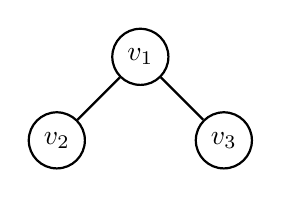
\begin{tikzpicture}[node distance={15mm}, thick, main/.style = {draw, circle}] 
\node[main] (1) {$v_1$}; 
\node[main] (2) [below left of=1] {$v_2$}; 
\node[main] (3) [below right of=1] {$v_3$}; 
\draw (1) -- (2); 
\draw (1) -- (3); 
\end{tikzpicture}
\caption{Interpersonal Connections among Voters} 
\label{fig:Figure0}
\end{figure}
\end{example}
We set the rising \( p \) value from 0 to 0.4, 0.6, and finally to 1. Through this small example, we observe that the winning committee changes. The \( p \) value can significantly influence the outcome of committee election results. Table \ref{tab:example_p_willingness} illustrates this phenomenon.

\begin{table}[ht]
\caption{Comparison of winning committees for different values of $p$}
\vspace{0.5cm} % Add vertical space after the caption
\centering
\begin{tabular}{ccccc}
 & $p = 0$ & $p = 0.4$ & $p = 0.6$ & $p = 1$ \\
candidates & $c_a$ \quad $c_b$ & $c_a$ \quad $c_b$ & $c_a$ \quad $c_b$ & $c_a$ \quad $c_b$ \\
\hline
$v_1$ & 0 \quad 1 & 0.4 \quad 0.6 & 0.6 \quad 0.4 &  1 \quad 0 \\
$v_2$ & 1 \quad 0 & 0.4 \quad 0.6 & 0.6 \quad 0.4 & 0 \quad 1 \\
$v_3$ &  1 \quad 0 & 0.6 \quad 0.4 &0.4 \quad 0.6 & 0 \quad 1 \\

sum & 2 \quad 1 & 1.6 \quad 1.4 & 1.4 \quad 1.6 & 1 \quad 2 \\
\hline
winning committee & $c_a$ & $c_a$ & $c_b$ & $c_b$ \\
\end{tabular}

\label{tab:example_p_willingness}
\end{table}


With this example, we can also observe that the score-based selfless rule is a special case of the score-based altruistic rule with \( p = 1 \), while the score-based selfish rule is a special case of the score-based altruistic rule with \( p = 0 \).





\subsection{Proof for weighted rules}
It's apparent that the altruistic voting rule we propose resembles a weighted voting rule. In this section, we provide a formal proof of this observation.

\subsubsection{Proof for score based altruistic rules}
\begin{lemma}
    Score based altruistic voting rule is a case of  weighted voting.
\end{lemma}

\begin{proof}
    
The calculation for score based altruistic rule is similar to the altruistic rule. According to   (\ref{SB:EQ_singlevoter_Score}) and    (\ref{SB:EQ_aggr_voter_Score})

\begin{equation*}
\begin{split}
s^{AL}(c) &= p \cdot \frac{1}{\vert F_{v_1}\vert}\big(f_{v_1}^{rel}(v_1)\beta_{v_1}(c) + \dots + f_{v_1}^{rel}(v_n)\beta_{v_n}(c)\big) + (1-p) \cdot \beta_{v_1}(c)\\
            &+ p \cdot \frac{1}{\vert F_{v_2}\vert}\big(f_{v_2}^{rel}(v_1)\beta_{v_1}(c) + \dots + f_{v_2}^{rel}(v_n)\beta_{v_n}(c)\big) + (1-p) \cdot \beta_{v_2}(c) \\
            &+ \dots \\ 
            &+ p \cdot \frac{1}{\vert F_{v_n}\vert}\big(f_{v_n}^{rel}(v_1)\beta_{v_1}(c) + \dots + f_{v_n}^{rel}(v_n)\beta_{v_n}(c)\big) +    (1-p) \cdot \beta_{v_n}(c)
\end{split}
\end{equation*}

And we can reformulate the equation:


\begin{equation*}
\begin{split}
s^{AL}(c) &= \beta_{v_1}(c)\big((1-p)+\frac{p}{\vert F_{v_1}\vert}(f_{v_1}^{rel}(v_1) +  \frac{p}{\vert F_{v_2}\vert}(f_{v_2}^{rel}(v_1)+ \dots +\frac{p}{\vert F_{v_n}\vert}(f_{v_n}^{rel}(v_1)\big) \\
            &+ \beta_{v_2}(c)\big((1-p)+\frac{p}{\vert F_{v_1}\vert}(f_{v_1}^{rel}(v_2) +  \frac{p}{\vert F_{v_2}\vert}(f_{v_2}^{rel}(v_2)+ \dots +\frac{p}{\vert F_{v_n}\vert}(f_{v_n}^{rel}(v_2)\big) \\
            &+  \dots  \\
            &+ \beta_{v_n}(c)\big((1-p)+\frac{p}{\vert F_{v_1}\vert}(f_{v_1}^{rel}(v_n) +  \frac{p}{\vert F_{v_2}\vert}(f_{v_2}^{rel}(v_n)+ \dots +\frac{p}{\vert F_{v_n}\vert}(f_{v_n}^{rel}(v_n)\big) 
\end{split}
\end{equation*}

The coefficient each voter has is only dependent on the structure of the voters. Therefore it is similar to the weighted voting rule.
\end{proof}

\section{Measuring altruism}
We devised an altruistic voting rule and sought to evaluate its effectiveness and impact. To achieve this, we required measurement methods to assess its performance. In this section, we developed various measurement methods for this purpose.
\subsection{Borda Score of a committee for a single voter}
In order to measure the altruism of the voting rules we proposed, we first need to calculate the Borda Score of a committee that a sigle voter gives. This score will show, to which extend can a chosen committee satisfes the preference of a voter. 
For calculation of the Borda Score of a committee in an election $E(C,V,k)$,  where $m = \vert C \vert, n= \vert V \vert$, we need as input, the preference ballot of each voter $\succeq_{v_i} \, \in \, \succeq$.  The Borda Scores $\beta_{v_i}(c_j)$ a candidate $c_j$ receives a from the voters $v_i$ according to (\ref{con:bordascore}) and  the friendship structure $F_{v_i}, where  \: i\leqslant n, j\leqslant m  \:and \:i, j \in \mathbb{N}$ and  the final voting outcome $C^{r} \in C$ of the applied voting rule $r$.  

We use the following equation to calculate the Borda Score of $v_i$ to the voted committee $C^{r}$ as a result of a voting rule r:
\begin{equation}
    \beta_{v_i}(C^{r}) = \sum_{c_i\in {C_{r}}}\beta_{v_i}(c_i)
\label{re:BordaScore_Committee}
\end{equation}

Using the equation \ref{re:BordaScore_Committee} we can calculate the SI of each voter. For example: 
\begin{equation*}
\begin{split}
     \beta_{v_1}(C^{r}) =\beta_{v_1}(c_a) + \beta_{v_1}(c_b)= 3
\end{split}\end{equation*}
Similarly, we can calculate $ \beta_{v_2}(C^{r}) = 3$, $ \beta_{v_3}(C^{r})=3$, $ \beta_{v_4}(C^{r})=1$. 

\subsection{Measuring altruism of each voter with the Average Friends Satisfaction Index (AvgFSI)}
After we defined the SI, we can use this value to evaluate the altruism of the applied voting rule. We suggest first to consider the average SI that a voter's friends have towards the final voting result after applying a certain voting rule $r$, we name this as Average Friends Satisfaction Index (AFSI). If we reach the result of $C^{r}$ in a committee election process using committee election rule $r$, for a voter $v_i$, to consider his whole friends circle $F_{v_i}$ and get the $I_{v_i}^{AvgFSI}$ as follows:  
\begin{equation}
     I_{v_i}^{AvgFSI}(C^{r}) = \frac{1}{\vert F_{v_i} \vert}\cdot \sum_{v_j\in {F_{v_i}}}  \beta_{v_j}(C^{r})   \label{si:AvgFSI}
\end{equation}

Concretely, we can consider the committee election example  $E(C,V,2)$,  where the candidates are $ C = \{c_a,c_b,c_c\}$, the voters are $V = \{v_1,v_2,v_3,v_4\}$  and $ m = 3, n = 4$ with the friend structure represented in Figure \ref{fig:Figure1}.  The preferences of the voters are respectively $\succeq_{v_1} =  \{c_a\succeq c_b \succeq c_c\}$,  $\succeq_{v_2} =  \{c_a\succeq c_b \succeq c_c\}$, $\succeq_{v_3} =  \{c_b\succeq c_a \succeq c_c\}$, $\succeq_{v_4} =  \{c_c\succeq c_a \succeq c_b\}$. The final result of the committee election $C^{r}= \{c_a, c_b\}$.

\begin{figure}[h]
\centering
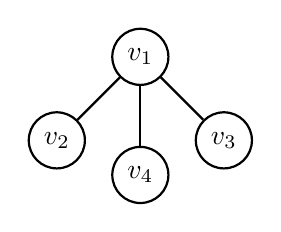
\begin{tikzpicture}[node distance={15mm}, thick, main/.style = {draw, circle}] 
\node[main] (1) {$v_1$}; 
\node[main] (2) [below left of=1] {$v_2$}; 
\node[main] (3) [below right of=1] {$v_3$}; 
\node[main] (4) [below of=1] {$v_4$}; 
\draw (1) -- (2); 
\draw (1) -- (3); 
\draw (1) -- (4); 
\end{tikzpicture}
\caption{Friends structure 2} \label{fig:Figure2}
\end{figure} 

Consider the example in Figure  \ref{fig:Figure2}.  We can calculate the AFSI of  $v_1$ as:
\begin{equation*}
    \begin{split}
     I_{v_1}^{AvgFSI}(C^{r}) &= \frac{1}{\vert F_{v_1} \vert}\cdot \sum_{v_j\in {F_{v_i}}}  \beta_{v_j}(C^{r})\\
                 &= \frac{1}{3}\cdot \big(  \beta_{v_2}(C^{r}) +  \beta_{v_3}(C^{r}) +  \beta_{v_4}(C^{r}) \big) =\frac{7}{3}
\end{split}
\end{equation*}

Similarly, we can calculate the other AFSI: $ I_{v_2}^{AvgFSI}(C^{r}) = I_{v_3}^{AvgFSI}(C^{r})=I_{v_4}^{AvgFSI}(C^{r}) = 3$.
We say, for a given committee election case, for a single voter, the higher AFSI a rule can bring, the higher the altruism level this voter give to this rule. 

\subsection{Measuring altruism of each voter with the Minimum Friends Satisfaction Index (MinFSI)}
It is also meaningful to find out the minimum satisfaction of in the voter's friends circle. For voter $v_i$ after applying a voting rule $r$ and reach the final result of $C^{r}$, we denote the Minimum Friends Satisfaction Index (Min-FSI) as $I_{v_i}^{MinFSI}(C^{r})$
\begin{equation}I_{v_i}^{MinFSI}(C^{r}) =  \min \big ( \{ \beta_{v}(C^{r}): v \in F_{v_i}\}  \big)\label{si:MinFSI}
\end{equation}
For our committee election case in Figure   \ref{fig:Figure1}, we can calculate $I_{v_1}^{MinFSI}(C^{r}) = 1$, $I_{v_2}^{MinFSI}(C^{r}) =3$, $I_{v_3}^{MinFSI}(C^{r}) = 3$ , $I_{v_4}^{MinFSI}(C^{r}) =3$.


\subsection{Measuring altruism of each voter with the Maximum Friends Satisfaction Index (MaxFSI)}

Similarly we can find out the maximum satisfaction of in the voter's friends circle. For voter
\begin{equation}I_{v_i}^{MaxFSI}(C^{r}) =  \max \big ( \{ \beta_{v}(C^{r}): v \in F_{v_i}\}  \big)\label{si:MaxFSI}
\end{equation}
For our committee election case in Figure   \ref{fig:Figure1}, we can calculate $I_{v_1}^{MaxFSI}(C^{r}) = 3$, $I_{v_2}^{MaxFSI}(C^{r}) =3$, $I_{v_3}^{MaxFSI}(C^{r}) = 3$ , $I_{v_4}^{MaxFSI}(C^{r}) =3$.



\subsection{Measuring the aggregated Satisfaction Index}
After we have considered the single voter FSI value, we now take a look at all voters aggregated and evaluate our voting rules also depending on the overall FSI scores.  For this, we will look at the different options shown in the table \ref{tab:aggregation_options}. In the chapter, we will introduce all these criterion one after another.


\begin{table}[h]
    \caption{Aggregation options}
    \vspace{0.5cm} % Add vertical space after the caption
    \centering
    \begin{tabular}{lccc}
\vspace{0.2cm}
 & Average(all) & Minimum(all) & Maximum(all) \\ 

       Average(single) & $I^{Avg-Avg}(C^{r})$ & $I^{Min-Avg}(C^{r})$ & $I^{Max-Avg}(C^{r})$ \\ 
   
        Minimum(single) & $I^{Avg-Min}(C^{r})$ & $I^{Min-Min}(C^{r})$ & $I^{Max-Min}(C^{r})$ \\ 

        Maximum(single) & $I^{Avg-Max}(C^{r})$ & $I^{Min-Max}(C^{r})$ & $I^{Max-Max}(C^{r})$ \\ 

    \end{tabular}

    \label{tab:aggregation_options}
\end{table}

We first consider the average, minimum and maximum of the AvgFSI of all voters for a voting rule $r$ in a committee election case $E(C,V,k)$,  where $m = \vert C \vert, n= \vert V \vert$. As we mentioned earlier, we denote $C^{r}$ as the final election result achieved by applying rule $r$:
\begin{equation}
     I^{Avg-Avg}(C^{r}) = \frac{1}{n}\cdot \sum_{j=1}^{n} I_{v_j}^{Avg}(C^{r})
\end{equation}\begin{equation}
     I^{Min-Avg}(C^{r}) = \min \big ( \{I_{v}^{Avg}(C^{r}): v \in V\}  \big) 
\end{equation}
\begin{equation}
     I^{Max-Avg}(C^{r}) = \max \big ( \{I_{v}^{Avg}(C^{r}): v \in V\}  \big) 
\end{equation}


For our committee election case in Figure   \ref{fig:Figure1}, we can calculate:
\begin{equation*}
 I^{Avg-Avg}(C^{r}) = \frac{17}{6},  I^{Min-Avg}(C^{r}) = \frac{7}{3},  I^{Max-Avg}(C^{r}) = 3
 \end{equation*}
Then we will consider the average, minimum and maximum of the MinFSI among all voters:

\begin{equation}
     I^{Avg-Min}(C^{r}) = \frac{1}{n}\cdot \sum_{j=1}^{n} I_{v_j}^{Min}(C^{r})
\end{equation}
\begin{equation}
     I^{Min-Min}(C^{r}) = \min \big ( \{I_{v}^{Min}(C^{r}): v \in V\}  \big) 
\end{equation}
\begin{equation}
     I^{Max-Min}(C^{r}) = \max \big ( \{I_{v}^{Min}(C^{r}): v \in V\}  \big) 
\end{equation}
For our committee election case in Figure   \ref{fig:Figure1}, we can calculate:

\begin{equation*}
 I^{Avg-Avg}(C^{r}) = \frac{5}{2}, I^{Min-Min}(C^{r}) = 1,  I^{Max-Min}(C^{r}) = 3
 \end{equation*}

Finally we will consider the average, minimum and maximum of the MaxFSI among all voters:
\begin{equation}
     I^{Avg-Max}(C^{r}) = \frac{1}{n}\cdot \sum_{j=1}^{n} I_{v_j}^{Max}(C^{r})
\end{equation}
\begin{equation}
     I^{Min-Max}(C^{r}) = \min \big ( \{I_{v}^{Max}(C^{r}): v \in V\}  \big) 
\end{equation}
\begin{equation}
     I^{Max-Max}(C^{r}) = \max \big ( \{I^{Max}(C^{r}): v \in V\}  \big) 
\end{equation}For our committee election case in Figure   \ref{fig:Figure1}, we can calculate:\begin{equation*}
    I^{Avg-Max}(C^{r}) = 3, I^{Min-Max}(C^{r}) = 3, I^{Max-Max}(C^{r}) = 3
\end{equation*}

\subsection{A concrete example to show the difference between the measurements}
In the election scenario, denoted as $E(C,V,3)$, the set of candidates is represented by $C = \{c_a,c_b,c_c,c_d,c_e,c_f\}$, and the set of voters is represented by $V = \{v_1,v_2,v_3,v_4,v_5,v_6\}$. The election has a committee size of $m = 6$, and a total of $n = 6$ voters. The friendship structure among the voters is illustrated in Figure \ref{fig:Figure2}. Each voter's preferences are as follows:


\begin{align*}
\succeq_{v_1} =  \{c_a\succeq c_b \succeq c_c\succeq c_d\succeq c_e\succeq c_f\},\\  \succeq_{v_2} =  \{c_b\succeq c_d \succeq c_e\succeq c_c\succeq c_f\succeq c_a\},\\ \succeq_{v_3} =  \{c_f\succeq c_e \succeq c_b\succeq c_a\succeq c_d\succeq c_c\}, \\\succeq_{v_4} =  \{c_d\succeq c_c \succeq c_a\succeq c_f\succeq c_b\succeq c_e\},\\\succeq_{v_1} =  \{c_c\succeq c_a \succeq c_f\succeq c_e\succeq c_d\succeq c_b\},\\\succeq_{v_1} =  \{c_e\succeq c_f \succeq c_d\succeq c_b\succeq c_a\succeq c_c\}. 
\end{align*}
\theoremstyle{definition}
\newtheorem{example1}{Example}[section]

\begin{example}
\begin{figure}[h]
\centering
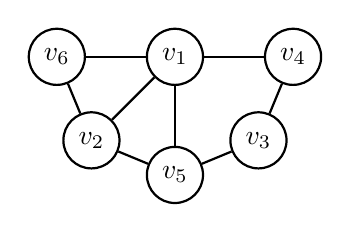
\begin{tikzpicture}[node distance={15mm}, thick, main/.style = {draw, circle}] 
\node[main] (1) {$v_1$}; 
\node[main] (2) [below left of=1] {$v_2$}; 
\node[main] (3) [below right of=1] {$v_3$}; 
\node[main] (4) [right of=1] {$v_4$}; 
\node[main] (5) [below of=1] {$v_5$}; 
\node[main] (6) [left of=1] {$v_6$}; 
\draw (1) -- (6); 
\draw (1) -- (2); 
\draw (1) -- (4); 
\draw (1) -- (5); 
\draw (2) -- (5); 
\draw (2) -- (6); 
\draw (3) -- (4); 
\draw (3) -- (5); 
\end{tikzpicture}
\caption{Friends structure 1 with 6 voters} \label{fig:Figure2}
\end{figure}

\begin{figure}[h]
\centering
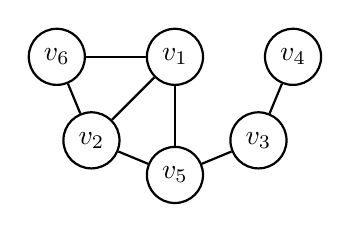
\begin{tikzpicture}[node distance={15mm}, thick, main/.style = {draw, circle}] 
\node[main] (1) {$v_1$}; 
\node[main] (2) [below left of=1] {$v_2$}; 
\node[main] (3) [below right of=1] {$v_3$}; 
\node[main] (4) [right of=1] {$v_4$}; 
\node[main] (5) [below of=1] {$v_5$}; 
\node[main] (6) [left of=1] {$v_6$}; 
\draw (1) -- (6); 
\draw (1) -- (2); 
\draw (1) -- (5); 
\draw (2) -- (5); 
\draw (2) -- (6); 
\draw (3) -- (4); 
\draw (3) -- (5); 
\end{tikzpicture}
\caption{Friends structure 2 with 6 voters} \label{fig:Figure3}
\end{figure}

Concretely we take an example with friends structure of Figure \ref{fig:Figure2}. We illustrate a friendship structure and demonstrate how all the measurements are to be calculated, with each yielding distinct results. 
\end{example}

We can start with calculating the Borda Score  and the single voter FSIs of the voted committee from each voter with Equations \ref{con:bordascore}, \ref{si:AvgFSI}, \ref{si:MinFSI}, \ref{si:MaxFSI}. 
With this example, we can find out that all of the proposed measuring means are of different types and can result in different values. 

We iterate throw all the possible committee in order to find the best committee under each measuring methods. We number the possible committee as follows:
    

\begin{table}[h]
\caption{List of all possible committees}
\vspace{0.5cm} % Add vertical space after the caption
\centering
\begin{tabular}{cccccc}
    $1. (c_a, c_b, c_c)$ & $2. (c_a, c_b, c_d)$ & $3.(c_a,c_b, c_e)$ & $4. (c_a, c_b, c_f)$ \\
    $5. (c_a, c_c,c_d)$ & $6. (c_a, c_c, c_e)$ & $7. (c_a, c_c, c_f)$ & $8. (c_a, c_d, c_e)$ \\
    $9. (c_a, c_d, c_f)$ & $10. (c_a, c_e, c_f)$ & $11. (c_b, c_c, c_d)$ & $12. (c_b, c_c, c_e)$ \\
    $13.(c_b, c_c, c_f)$ & $14. (c_b, c_d, c_e)$ & $15.(c_b, c_d, c_f)$ & $16. (c_b, c_e, c_f)$ \\
    $17. (c_c, c_d, c_e)$ & $18.(c_c, c_d, c_f)$ & $19. (c_c, c_e, c_f)$ & $20.(c_d, c_e, c_f)$ \\
\end{tabular}
\label{tab:my_label}
\end{table}

If we consider the friends structure of Figure \ref{fig:Figure2}. We can use the 9 measuring methods and come to the conclusion that for each of these methods, the following committee will be the best committee as in Table \ref{tab:res_table_1}:
\begin{table}[h] 
\caption{Ideal committee - committee number - structure 1 }
\vspace{0.5cm} % Add vertical space after the caption
\centering
\begin{tabular}{ccc}
    \multicolumn{3}{c}{\textbf{Structure 1}} \\
    \hline
    $avg-avg$ & $min-avg$ & $max-avg$ \\
    0 & 11 & 0 \\
    $avg-min$ & $min-min$ & $max-min$ \\
    1 & 7 & 0 \\
    $avg-max$ & $min-max$ & $max-max$ \\
    0 & 4 & 1 \\
\end{tabular}
\label{tab:res_table_1}
\end{table}

\begin{table}[h]
\caption{Ideal committee - committee number - structure 2}
\vspace{0.5cm} % Add vertical space after the caption
\centering
\begin{tabular}{ccc}
    \multicolumn{3}{c}{\textbf{Structure 2}} \\
    \hline
    $avg-avg$ & $min-avg$ & $max-avg$ \\
    3 & 15 & 15 \\
    $avg-min$ & $min-min$ & $max-min$ \\
    0 & 15 & 11 \\
    $avg-max$ & $min-max$ & $max-max$ \\
    0 & 12 & 7 \\
\end{tabular}
\label{tab:res_table_2}
\end{table}


  

This way, we can find out that all of these methods are optimising to different results and are not dependent of each other.


\subsection{Finding the best committee as ILP Problems}

To find the best committee for the different measuring methods can be very time consuming. Therefore we want to turn them into ILP problems and user existing solver Gurobi to accelerate the calculation. For measuring methods "Max-Max", "Max-Min", "Max-Avg", we developed for each voter an ILP model and gather the result of all voters to find the best value. For the rest of the measuring methods, we developed one corresponding ILP model. All our ILP models will be explained in this chapter. All ILP models have a the following common input:

\paragraph*{Common Input}
\begin{itemize}
  \item \textbf{Input}:
A committee election case $E (C,V,k)$ where $\vert C \vert =m $, $\vert V \vert =n$, A graph $G(V,E)$ to represent the relationship between the voters and the preference of each voter towards all candidates.
\end{itemize}
\paragraph*{ILP Problem 1: Maximizing  $I^{Avg-Avg}(C^{r})$}
\
\begin{itemize}
  \item \textbf{Variables}: 

\textbf{A set of binary decision variables $x_i$:} \[  x_i \in \{0, 1\} , \,\, i=1,2,\dots, m \] The value of $x_i$ represents the status of candidate $c_i$, \(x_i = 1\) indicates choosing $c_i$ and \(x_i = 0\) indicates not choosing $c_i$.


\textbf{A continuous decision variables $s$:} 
\[  s\in \mathbb{Q}_{\geq 0} \]  
$s$ represents the value of $I^{Avg-Avg}(C^{r})$.
    \item \textbf{Constraints}:
The constraint requires that the sum of binary decision variables \(x_1, x_2, \ldots, x_m\) equals the committee size of the election \(k\), represented as:
\begin{equation} \sum_{i=1}^m x_i = k     \label{eq:ilpavgavg1}
\end{equation}

To constraint $s$:
\begin{equation}
s \leq \frac{1}{n}\cdot \sum_{j=1}^{n} \beta_{v_j}^{Avg}(C^{r})
\end{equation}
  
  \item  \textbf{Objective function:}
  \[\text{maximize} \quad s\]

 \item  \textbf{Explanation:}
Constraint \ref{eq:ilpavgavg1} ensures that the number of selected candidates in the committee \(C^r\) is exactly \(k\). This constraint guarantees that the committee size is fixed and meets the required number of candidates. \(s\) represents the value of $I^{Avg-Avg}(C^{r})$ if a preferred committee \(C^r\) is to win the election. Maximizing \(s\) in a feasible ILP solution ensures that \(s\) provides the maximum value of \(I^{Avg-Avg}(C^{r})\). 

If there exists a feasible solution to this ILP where all constraints are satisfied and \(s\) is maximized, then \(s\) will indeed give us the maximum value of \(I^{Avg-Avg}(C^{r})\). This means that the selected committee \(C^r\) optimally meets the requirements set by the ILP formulation, ensuring both the fixed committee size \(k\) and the maximum of the average FSI. 
\end{itemize}

\paragraph*{ILP Problem 2: Maximizing $I^{Min-Avg}(C^{r})$}\mbox{} \\

\begin{itemize}
  \item \textbf{Variables}: 

\textbf{A set of binary decision variables $x_i$:} \[  x_i \in \{0, 1\} , \,\, i=1,2,\dots, m \] The value of $x_i$ represents the status of candidate $c_i$, \(x_i = 1\) indicates choosing $c_i$ and \(x_i = 0\) indicates not choosing $c_i$.


\textbf{A continuous decision variables $s$:} 
\[  s\in \mathbb{Q}_{\geq 0} \] 
$ \forall v_j \in V s$ represents the value of $I_{v_j}^{Avg}(C^{r})$.
    \item \textbf{Constraints}:
The constraint requires that the sum of binary decision variables \(x_1, x_2, \ldots, x_m\) equals the committee size of the election \(k\), represented as:
\begin{equation} \sum_{i=1}^m x_i = k     \label{eq:ilpminavg1}
\end{equation}

To further constraint $s$, for all $v_j$ the following constraint inequality holds:
\begin{equation}\forall v_j \in V, \quad s \leq \beta_{v_j}^{Avg}(C^{r})    \label{eq:ilpminavg2}
\end{equation}
  
  \item  \textbf{Objective function:}
  \[\text{maximize} \quad s\]





 \item  \textbf{Explanation:}
Constraint \ref{eq:ilpminavg1} ensures that the number of selected candidates in the committee \(C^r\) is exactly \(k\). This constraint guarantees that the committee size is fixed and meets the required number of candidates. 

\(s\) serves as the lower bound of $I^{Min-Avg}(C^{r})$ if a preferred committee \(C^r\) is to win the election. Constraint \ref{eq:ilpminavg2} ensures that $s$ is the lower bound of all \(I_{v_j}^{Avg}(C^{r})\). Maximizing \(s\) in a feasible ILP solution ensures that \(s\) provides the maximum value of \(I^{Min-Avg}(C^{r})\). 

If there exists a feasible solution to this ILP where all constraints are satisfied and \(s\) is maximized, then \(s\) will indeed give us the maximum value of \(I^{Min-Avg}(C^{r})\). This means that the selected committee \(C^r\) optimally meets the requirements set by the ILP formulation, ensuring both the fixed committee size \(k\) and the minimum of the average FSI. 






\end{itemize}
















\paragraph*{ILP Problem 3: Maximizing  $I^{Avg-Max}(C^{r})$}

\begin{itemize}

  \item \textbf{Variables}: 

\textbf{A set of binary decision variables $x_i$:} \[  x_i \in \{0, 1\} , \,\, i=1,2,\dots, m \] The value of $x_i$ represents the status of candidate $c_i$, \(x_i = 1\) indicates choosing $c_i$ and \(x_i = 0\) indicates not choosing $c_i$.


\textbf{A set of two-dimensional binary decision variables \( a_{yj} \):}
\[
\{ a_{yj} \mid 1 \leq j \leq n, \quad 1 \leq y \leq |F_{v_j}| \},  \quad (j, y \in \mathbb{N})
\]

\textbf{A set of continuous decision variables $s_j$:} 
 \[  s_j\in \mathbb{Q}_{\geq 0}, \quad j=1,2, \dots,n \] 
$s_j$ represents the value of $I_{v_j}^{MaxFSI}$ of \(v_j\).
    \item \textbf{Constraints}:
The constraint requires that the sum of binary decision variables \(x_1, x_2, \ldots, x_m\) equals the committee size of the election \(k\), represented as:
\begin{equation} \sum_{i=1}^m x_i = k \label{eq:ilpavgmax1}
\end{equation}

For each \(j\) with \(1 \leq j \leq |V|\), the constraint is that the sum of \( a_{yj} \) for all \( x \in F_{v_j} \) (where \( v_j \) belongs to the set \( V \)) equals 1.:
\begin{equation} \forall j \in \{1, 2, \ldots, |V|\}, \quad \sum_{y=1}^{|F_{v_j}|} a_{yj} = 1 \label{eq:ilpavgmax2}
\end{equation}

To further constraint $s_j$ as the $I_{v_j}^{MaxFSI}$, we introduce a very big value $M$, in our case $M \geq  2m$. For all \( j \in \{1, 2, \ldots, |V|\} \) and for each  \( y \in \{1, 2, \ldots, |\text{F}_{v_j}|\} \), the following constraint inequality holds:
\begin{equation} \forall v_y \in F_{v_j}, \,  \forall v_j \in V :\quad \beta_{v_y}(C^{r}) + (1 - a_{yj})\cdot M \geq s_j \label{eq:ilpavgmax3}
\end{equation}
  
  \item  \textbf{Objective function:}
  \begin{equation}\text{maximize} \quad \frac{\sum_{i=1}^{n} s_j}{n}    \label{eq:ilpavgmax4}
\end{equation}


\item  \textbf{Explanation:}
Constraint \ref{eq:ilpavgmax1} ensures that the number of selected candidates in the committee \(C^r\) is exactly \(k\). This constraint guarantees that the committee size is fixed and meets the required number of candidates.
Constraint \ref{eq:ilpavgmax2} guarantees that only one friend of each voter is selected for getting the maximized FSI.
Constraint \ref{eq:ilpavgmax3} indicates that \(s\) serves as an upper bound of the highest FSI given by a voter's friend if a preferred committee \(C^r\) wins the election.
The objective function \ref{eq:ilpavgmax4} represents the $I^{Avg-Max}(C^{r})$ over all voters. Maximizing the objective function in a feasible ILP solution ensures that the ILP provides the maximum value of \(I^{Avg-Max}(C^{r})\), representing the average FSI among the most satisfied friends of each voter given by a winning committee \(C^r\)in the election. 

If there exists a feasible solution to this ILP where all constraints are satisfied and the objective function is maximized, then the ILP will indeed give us the maximum value of \(I^{Avg-Max}(C^{r})\). This means that the selected committee \(C^r\) optimally meets the requirements set by the ILP formulation, ensuring both the fixed committee size \(k\) and is the upper bound of the average FSI value of the most satisfied friends. 

\end{itemize}


\paragraph*{ILP Problem 4: Maximizing  $I^{Max-Max}(C^{r})$}\mbox{} \\

For this we will do the optimization of the $I_{v_i}^{Max}(C^{r})$ for each voter $v_i$. Afterwards, we will iterate through all the $I_{v_i}^{Max}(C^{r})$ and find the maximum value:
  \[I^{Max-Max}(C^{r}) = \max\{ I_{v_1}^{Max}(C^{r}), I_{v_2}^{Max}(C^{r}), \ldots, I_{v_n}^{Max}(C^{r}) \}\]
\begin{itemize}

  \item \textbf{Variables}: 

\textbf{A set of binary decision variables $x_i$:}\[  x_i \in \{0, 1\} , \,\, i=1,2,\dots, m \] The value of $x_i$ represents the status of candidate $c_i$, \(x_i = 1\) indicates choosing $c_i$ and \(x_i = 0\) indicates not choosing $c_i$.


\textbf{A set of two-dimensional binary decision variables \( a_{yj} \):}
\[
\{ a_{yj} \mid 1 \leq j \leq n, \quad 1 \leq y \leq |F_{v_j}| \},  \quad (j, y \in \mathbb{N})
\]

\textbf{A continuous decision variables $s$:} 
\[  s\in \mathbb{Q}_{\geq 0} \] 
$s$ represents the value of $I^{Max-Max}$ .
    \item \textbf{Constraints}:
The constraint requires that the sum of binary decision variables \(x_1, x_2, \ldots, x_m\) equals the committee size of the election \(k\), represented as:
\begin{equation} \sum_{i=1}^m x_i = k     \label{eq:ilpmaxmax1}
\end{equation}

For each \(j\) with \(1 \leq j \leq |V|\), the constraint is that the sum of \( a_{yj} \) for all \( x \in F_{v_j} \) (where \( v_j \) belongs to the set \( V \)) equals 1.:
\begin{equation} \forall j \in \{1, 2, \ldots, |V|\}, \quad \sum_{y=1}^{|F_{v_j}|} a_{yj} = 1 \label{eq:ilpavgmax2}
\end{equation}

To further constraint $s$ as the $I^{Max-Max}$, we introduce a very big value $M$, in our case $M \geq  2m$. For all \( j \in \{1, 2, \ldots, |V|\} \) and for each  \( y \in \{1, 2, \ldots, |\text{F}_{v_j}|\} \), the following constraint inequality holds:
\begin{equation} \forall v_y \in F_{v_j}, \,  \forall v_j \in V :\quad \beta_{v_y}(C^{r}) + (1 - a_{yj})\cdot M \geq s \label{eq:ilpavgmax3}
\end{equation}
  
  \item  \textbf{Objective function:}
  \[\text{maximize} \quad s \]

\item  \textbf{Explanation:}
Constraint \ref{eq:ilpmaxmax1} ensures that the number of selected candidates in the committee \(C^r\) is exactly \(k\). This constraint guarantees that the committee size is fixed and meets the required number of candidates.
Constraint \ref{eq:ilpmaxmax2} guarantees that only one friend of each voter is selected for getting the maximized FSI.
Constraint \ref{eq:ilpmaxmax3} indicates that \(s\) represents the upper bounded FSI given by a voter's friend if a preferred committee \(C^r\) win the election. Maximizing \(s\) in a feasible ILP solution ensures that \(s\) provides the maximum value of \(I_{v_i}^{Max}(C^{r})\), representing the maximun FSI a voter can reach given by a winning committee \(C^r\)in the election. 

If there exists a feasible solution to this ILP where all constraints are satisfied and \(s\) is maximized, then \(s\) will indeed give us the maximum value of \(I_{v_i}^{Max}(C^{r})\). This means that the selected committee \(C^r\) optimally meets the requirements set by the ILP formulation, ensuring both the fixed committee size \(k\) and the maximum of the most satisfied friends. Afterwards, we gether the result for each voter $v_i$ and retrieve the highest score among all voters. This will give the $I^{Max-Max}(C^{r})$ over all voters.

\end{itemize}


\paragraph*{ILP Problem 5: Maximizing  $I^{Avg-Min}(C^{r})$}

\begin{itemize}

  \item \textbf{Variables}: 

\textbf{A set of binary decision variables $x_i$:} \[  x_i \in \{0, 1\} , \,\, i=1,2,\dots, m \] The value of $x_i$ represents the status of candidate $c_i$, \(x_i = 1\) indicates choosing $c_i$ and \(x_i = 0\) indicates not choosing $c_i$.

\textbf{A set of continuous decision variables $s_j$:} 
\[   s_j\in \mathbb{Q}_{\geq 0}  \quad j=1,2,\dots,n \] 
$s_i$ represents the value of $I_{v_i}^{MinFSI}$ of \(v_i\).
    \item \textbf{Constraints}:
The constraint requires that the sum of binary decision variables \(x_1, x_2, \ldots, x_m\) equals the committee size of the election \(k\), represented as:
\begin{equation} \sum_{i=1}^m x_i = k \label{eq:ilpavgmin1}
\end{equation}

To further constraint $s_j$, the following constraint inequality holds:
\begin{equation} \forall v_y \in F_{v_j}, \,  \forall v_j \in V :\quad \beta_{v_y}(C^{r}) \geq s_j  \label{eq:ilpavgmin2}
\end{equation}
  
  \item  \textbf{Objective function:}
  \begin{equation}\text{maximize} \quad \frac{\sum_{j=1}^{n} s_j}{n} \label{eq:ilpavgmin3}
\end{equation}
\item  \textbf{Explanation:}
Constraint \ref{eq:ilpavgmin1} ensures that the number of selected candidates in the committee \(C^r\) is exactly \(k\). This constraint guarantees that the committee size is fixed and meets the required number of candidates.
Constraint \ref{eq:ilpavgmin2} indicates that \(s\) serves as a lower bound of each voter's FSI given by all his friends if a preferred committee \(C^r\) win the election.
The objective function \ref{eq:ilpavgmin3} represents the average of the $I^{Min}(C^{r})$ over all voters. Maximizing  the objective function in a feasible ILP solution ensures that the ILP provides the maximum value of \(I^{Avg-Min}(C^{r})\), representing the average FSI among the least satisfied friends of each voter given by the chosen committee \(C^r\)in the election. 

If there exists a feasible solution to this ILP where all constraints are satisfied and the objective function is maximized, then the ILP will indeed give us the maximum value of \(I^{Avg-Min}(C^{r})\). This means that the selected committee \(C^r\) optimally meets the requirements set by the ILP formulation, ensuring both the fixed committee size \(k\) and is the average of the least satisfied friends. 
\end{itemize}


\paragraph*{ILP Problem 6: Maximizing  $I^{Min-Max}(C^{r})$}

\begin{itemize}

  \item \textbf{Variables}: 

\textbf{A set of binary decision variables $x_i$:} \[  x_i \in \{0, 1\} , \,\, i=1,2,\dots, m \] The value of $x_i$ represents the status of candidate $c_i$, \(x_i = 1\) indicates choosing $c_i$ and \(x_i = 0\) indicates not choosing $c_i$.


\textbf{A set of two-dimensional binary decision variables \( a_{yj} \):}
\[
\{ a_{yj} \mid 1 \leq j \leq n, \quad 1 \leq y \leq |F_{v_j}| \},  \quad (j, y \in \mathbb{N})
\]

\textbf{A set of continuous decision variables $s$:} 
\[  s\in \mathbb{Q}_{\geq 0} \] 
$s$ represents the value of $I^{Min-Max}$ .
    \item \textbf{Constraints}:
The constraint requires that the sum of binary decision variables \(x_1, x_2, \ldots, x_m\) equals the committee size of the election \(k\), represented as:
\begin{equation} \sum_{i=1}^m x_i = k  \label{eq:ilpminmax1}
\end{equation}

For each \(i\) with \(1 \leq i \leq |V|\), the constraint is that the sum of \( a_{ij} \) for all \( j \in F_{vi} \) (where \( i \) belongs to the set \( V \)) equals 1.:
\begin{equation} \forall j \in \{1, 2, \ldots, |V|\}, \quad \sum_{y=1}^{|F_{v_j}|} a_{yj} = 1  \label{eq:ilpminmax2}
\end{equation}

To further constraint $s$ as the $I^{Min-Max}$, we introduce a very big value $M$, in our case $M \geq  2m$. For all \( j \in \{1, 2, \ldots, |V|\} \) and for each  \( y \in \{1, 2, \ldots, |\text{F}_{v_j}|\} \), the following constraint inequality holds:
\begin{equation}  \forall v_y \in F_{v_j}, \,  \forall v_j \in V :\quad \beta_{v_y}(C^{r}) + (1 - a_{yj})\cdot M \geq s      \label{eq:ilpminmax3}
\end{equation}
  
  \item  \textbf{Objective function:}
  \[\text{maximize} \quad s \]

\item  \textbf{Explanation:}
Constraint \ref{eq:ilpminmax1} ensures that the number of selected candidates in the committee \(C^r\) is exactly \(k\). This constraint guarantees that the committee size is fixed and meets the required number of candidates.
Constraint \ref{eq:ilpminmax2} guarantees that only one friend of each voter is selected for getting the maximized FSI.
Constraint \ref{eq:ilpminmax3} indicates that \(s\) serves as a lower bound on the highest FSI given by any voter's friend if a preferred committee \(C^r\) win the election. Maximizing \(s\) in a feasible ILP solution ensures that \(s\) provides the maximum value of \(I^{Min-Max}(C^{r})\), representing the minimum FSI among the most satisfied friends of each voter given by a winning committee \(C^r\)in the election. 

If there exists a feasible solution to this ILP where all constraints are satisfied and \(s\) is maximized, then \(s\) will indeed give us the maximum value of \(I^{Min-Max}(C^{r})\). This means that the selected committee \(C^r\) optimally meets the requirements set by the ILP formulation, ensuring both the fixed committee size \(k\) and the minimum of the most satisfied friends. In this case, we make the FSI score among the most satisfied friends retain a highest possible FSI score.
\end{itemize}

\paragraph*{ILP Problem 7: Maximizing  $I^{Min-Min}(C^{r})$}

\begin{itemize}

  \item \textbf{Variables}: 

\textbf{A set of binary decision variables $x_i$:} \[  x_i \in \{0, 1\} , \,\, i=1,2,\dots, m \] The value of $x_i$ represents the status of candidate $c_i$, \(x_i = 1\) indicates choosing $c_i$ and \(x_i = 0\) indicates not choosing $c_i$.

\textbf{A continuous decision variables $s$:} 
\[  s\in \mathbb{Q}_{\geq 0} \]  
$s$ represents the value of $I^{Min-Min}$ .
    \item \textbf{Constraints}:
The constraint requires that the sum of binary decision variables \(x_1, x_2, \ldots, x_m\) equals the committee size of the election \(k\), represented as:

\begin{equation} \sum_{i=1}^m x_i = k     \label{eq:ilpminmin1}
\end{equation}


To further constraint $s$, assuming $C^r$ is every possible committee in the size of $k$, the following constraint inequality holds:
\begin{equation}   \forall v_y \in F_{v_j}, \,  \forall v_j \in V :\quad \beta_{v_y}(C^{r}) \geq s        \label{eq:ilpminmin2}
\end{equation}

  
  \item  \textbf{Objective function:}
  \[\text{maximize} \quad s \]

 \item  \textbf{Explanation:}
Constraint \ref{eq:ilpminmin1} ensures that the number of selected candidates in the committee \(C^r\) is exactly \(k\). This constraint guarantees that the committee size is fixed and meets the required number of candidates.

Constraint \ref{eq:ilpminmin2} indicates that \(s\) serves as a lower bound on the lowest FSI required by any voter's friend preferred committee \(C^r\) to win the election, based on voter preferences. Maximizing \(s\) in a feasible ILP solution ensures that \(s\) provides the maximum value of \(I^{Min-Min}(C^{r})\), representing the minimum FSI of the least satisfied friend among all voters of a winning committee \(C^r\)in the election. 

If there exists a feasible solution to this ILP where all constraints are satisfied and \(s\) is maximized, then \(s\) will indeed give us the maximum value of \(I^{Min-Min}(C^{r})\). This means that the selected committee \(C^r\) optimally meets the requirements set by the ILP formulation, ensuring both the fixed committee size \(k\) and the minimum of the least satisfied friends. In this case, we make the least satisfied friend, as happy as possible.
\end{itemize}
\paragraph*{ILP Problem 8: Maximizing  $I^{Max-Min}(C^{r})$}\mbox{} \\
For this we will do the optimization of the $I_{v_i}^{Min}(C^{r})$ for each voter $v_i$. Afterwards, we will iterate through all the $I_{v_i}^{Min}(C^{r})$ and find the maximum value:
  \[I^{Max-Min}(C^{r}) = \max\{ I_{v_1}^{Min}(C^{r}), I_{v_2}^{Min}(C^{r}), \ldots, I_{v_n}^{Min}(C^{r}) \}\]
\begin{itemize}
  \item \textbf{Variables}: 

\textbf{A set of binary decision variables $x_i$:} \[  x_i \in \{0, 1\} , \,\, i=1,2,\dots, m \] The value of $x_i$ represents the status of candidate $c_i$, \(x_i = 1\) indicates choosing $c_i$ and \(x_i = 0\) indicates not choosing $c_i$.


\textbf{A continuous decision variables $s$:} 
\[  s\in \mathbb{Q}_{\geq 0} \] 
$s$ represents the value of $I_{v_i}^{MinFSI}$.
    \item \textbf{Constraints}:
The constraint requires that the sum of binary decision variables \(x_1, x_2, \ldots, x_m\) equals the committee size of the election \(k\), represented as:
\begin{equation} \sum_{i=1}^m x_i = k     \label{eq:ilpmaxmin1}
\end{equation}

To further constraint $s$, for all $ v_y $ in $F_{v_j} $ the following constraint inequality holds:
\begin{equation} \forall v_y \in F_{v_j}, \,  \forall v_j \in V :\quad \beta_{v_y}(C^{r}) \geq s   \label{eq:ilpmaxmin2}
\end{equation}
  
  \item  \textbf{Objective function:}
  \[\text{maximize} \quad s\]

  \item  \textbf{Explanation:}
Constraint \ref{eq:ilpmaxmin1} ensures that the number of selected candidates in the committee \(C^r\) is exactly \(k\). This constraint guarantees that the committee size is fixed and meets the required number of candidates.

Constraint \ref{eq:ilpmaxmin2} indicates that \(s\) serves as a lower bound of the smallest FSI given by each friend of the voter if a preferred committee \(C^r\) to win the election. Maximizing \(s\) in a feasible ILP solution ensures that \(s\) provides the maximum value of \(I_{v_i}^{Min}(C^{r})\), representing the minimum FSI of the least satisfied friend of $v_i$. 

If there exists a feasible solution to this ILP where all constraints are satisfied and \(s\) is maximized, then \(s\) will indeed give us the maximum value of  \(I_{v_i}^{Min}(C^{r})\). This means that the selected committee \(C^r\) optimally meets the requirements set by the ILP formulation, ensuring both the fixed committee size \(k\) and the minimum of the FSI. Afterwards, we gether the result for each voter $v_i$ and retrieve the highest score among all voters. This will give the $I^{Max-Min}(C^{r})$ over all voters.
\end{itemize}

\paragraph*{ILP Problem 9: Maximizing  $I^{Max-Avg}(C^{r})$}\mbox{} \\
For this we will do the optimization of the $I_{v_j}^{Avg}(C^{r})$ for each voter $v_j$. Afterwards, we will iterate through all the $I_{v_j}^{Avg}(C^{r})$ and find the maximum value:
  \[I^{Max-Avg}(C^{r}) = \max\{ I_{v_1}^{Avg}(C^{r}), I_{v_2}^{Avg}(C^{r}), \ldots, I_{v_n}^{Avg}(C^{r}) \}\]
\begin{itemize}
  \item \textbf{Variables}: 

\textbf{A set of binary decision variables $x_i$:} \[  x_i \in \{0, 1\} , \,\, i=1,2,\dots, m \] The value of $x_i$ represents the status of candidate $c_i$, \(x_i = 1\) indicates choosing $c_i$ and \(x_i = 0\) indicates not choosing $c_i$.


\textbf{A continuous decision variables $s$:} 
\[  s\in \mathbb{Q}_{\geq 0} \] 
$s$ represents the value of $I_{v_j}^{Avg}(C^{r})$ and can therefore be reformulated as follows:
\[ s \leq I_{v_j}^{Avg}(C^{r})\]
    \item \textbf{Constraints}:
The constraint requires that the sum of binary decision variables \(x_1, x_2, \ldots, x_m\) equals the committee size of the election \(k\), represented as:
\begin{equation} \sum_{i=1}^m x_i = k     \label{eq:ilpmaxavg1}
\end{equation}
  
  \item  \textbf{Objective function:}
  \[\text{maximize} \quad s\]

  \item  \textbf{Explanation:}
Constraint \ref{eq:ilpmaxavg1} ensures that the number of selected candidates in the committee \(C^r\) is exactly \(k\). This constraint guarantees that the committee size is fixed and meets the required number of candidates.

For each $v_j$, \(s\) serves as $I_{v_j}^{Avg}(C^{r})$ given by all friends of the $v_j$ if a preferred committee \(C^r\) is to win the election. Maximizing \(s\) in a feasible ILP solution ensures that \(s\) provides the maximum value of \(I_{v_j}^{Avg}(C^{r})\), representing the maximum of the average FSI if all friends of $v_j$. 

If there exists a feasible solution to this ILP where all constraints are satisfied and \(s\) is maximized, then \(s\) will indeed give us the maximum value of  \(I_{v_j}^{Avg}(C^{r})\). This means that the selected committee \(C^r\) optimally meets the requirements set by the ILP formulation, ensuring both the fixed committee size \(k\) and the maximum of the average FSI. Afterwards, we gather the result for each voter $v_j$ and retrieve the highest score among all voters. This will give the $I^{Max-Avg}(C^{r})$ over all voters.

\end{itemize}


\section{The friend structure represented by graph models}

The Erdős–Rényi (ER) model was chosen to generate the friendship structure between voters because of several reasons. Firstly, the ER model, denoted as $G(n,p)$, is straightforward and intuitive, making it easy to understand, especially for readers unfamiliar with network science. Additionally, the ER model allows me to control the rising density of the generated graph by adjusting the probability parameter $p$, providing flexibility in exploring various network densities.

Moreover, the ER model is widely used and extensively studied in the field of network science. Its properties and behavior have been well documented, enabling comprehensive analysis and interpretation of the generated social structures. By leveraging the ER model, I can draw upon existing literature and methodologies to analyze the friendship networks between voters more effectively.

Furthermore, my thesis explores the concept of altruistic voting, which represents a relatively newly studied field in preference modeling. Given the exploratory nature of this research area, the ER model serves as a suitable starting point for investigating the underlying social structures and dynamics of altruistic voting behavior. Its simplicity and versatility allow me to lay the foundation for more sophisticated analyses and modeling approaches in future research.

Overall, the ER model provides a solid framework for generating and analyzing friendship networks between voters, offering both simplicity and versatility that align well with the objectives of my thesis on altruistic voting behavior.

With the voter data from \href{https://www.preflib.org}{PrefLib}, we can extract an election $E (C,V,k)$ and the preference of each voter over all the candidates. We use the Erdős–Rényi (ER) model to generate a friendship structure randomly. For a graph $G(p,n)$, the nodes correspond to each of the voters, and the friendship between voters is represented by edges. If two voters are friends, there will be an edge between them. For example, in the \href{https://www.preflib.org/static/data/agh/00009-00000001.soc}{AGH Course Selection 2003}, 146 students provided a Complete List of Strict Orders from 9 candidate courses. For this, we can generate a graph model $G(p,146)$ with $p \in [0,1]$. We can define the $p$ value depending on the different settings of our experiment in the coming sections.


\section{The research experiment}
In the previous chapter, we examined a single example where the results obtained from the 9 measuring methods were different.  However, this observation may be specific to that particular instance. To generalize our findings and gain a deeper understanding, we need to analyze a larger set of examples using these 9 methods. By conducting a quantitative analysis across multiple scenarios, we can effectively compare the measuring methods.
\subsection{Research Questions}
With the measuring methods designed and the ILP models ready. We do a data analysis experiment with data instances from \href{https://www.preflib.org/}{PrefLib} in our next step. Our measuring methods are designed for instances of type SOC (Strict Orders - Complete List). We will consider the FIS for the 9 different measuring methods separately and do not mix their results. Our research questions are listed as follows:
\begin{enumerate}
    \item \textbf{Research Question 1}: How likely are the 9 methods to be different from each other?
        \newline
    For this, we will fix the PrefLib instance and the committee size and the graph type. With growing $p$ in the range $[0.1,1]$, we will compare each pair of the measuring methods and observe whether the result committee is identical or not.
    \item \textbf{Research Question 2}: Given a graph type representing the relationship between all the voters, how will the density of the graph influence the FSI values. 
    \newline
For this experiment, we will fix the graph type, the committee size for the election, and the PrefLib instance. We will observe the development of the FSI (Friendship Strength Index) value under different measurement methods with growing $p$ in the range $[0.1,1]$. Here, $p$ represents the probability parameter in the Erdős–Rényi (ER) model, denoted as $G(n,p)$, which we mentioned above.

    
    \item \textbf{Research Question 3}: How does the increasing willingness, represented by the rising proportion \( p \), in our altruistic voting rule affect the FSI value of all nine methods?

    To address this question, we will load the PrefLib instances and generate the friendship structures using random graphs. Subsequently, we will conduct experiments by varying the committee size and the \( p \) value. We will observe the changes in the FSI value under different measurement methods, considering varying graph densities: dense (edges probability greater than 0.5) and not dense (edges probability less than 0.5). Detailed assumptions and experimental results will be presented and explained in the corresponding section.

\end{enumerate}

\subsection{Hardware and Software Setups and Utilization for the Experiment}

As an integral component of my master's thesis project, I utilized the Linux server provided by TU Clausthal for experimentation purposes. This server, equipped with 128GB of RAM and an advanced CPU configuration as of 2023, served as the computational backbone for executing various algorithms, simulations, and data processing tasks crucial to my research. Throughout the project, the Linux server played a pivotal role in processing datasets, solving ILP models, and conducting computational tasks that required significant memory and processing resources. For coding tasks, I primarily used Python, and for data storage, I employed MongoDB. Additionally, ILP models were solved using the Gurobi solver.

\subsection{Data Acquisition}
The experiment utilized .soc data samples sourced from the PrefLib dataset. A total of 200 preference data samples for question 1 and 2 nd 300 were chosen for question 3 for our experiment and analysis, determined by computational constraints. This sample size was deemed manageable within the researcher's computational capability. Each data sample encompasses voter information, candidate details, and individual voter preferences toward all candidates, represented with strict order and completeness in the .soc format. Borda scores were then assigned to each candidate based on the aggregated voter preferences. Additionally, the friendship structure was simulated through random graph generation using the Erdős–Rényi (ER) model, with the graph size determined by the number of voters in each data sample. 

\subsection{Experiment - Research Question 1 and 2}


\paragraph*{Implementation of ILP Models for Ideal Committee}\mbox{} \\
For the experiment, ILP models were implemented for nine measuring methods using the Gurobi optimization library in Python. These models were used to determine the ideal winning committee and the corresponding ILP values with varying committee sizes from $1$ to $m-1$, where $m$ represents the total number of candidates. Additionally, the density of the random graph representing the friendship structure among candidates was incrementally increased from 0.1 to 1 in steps of 0.1. 

We computed the optimal value and corresponding winning committee for each measurement method applied to every data sample from PrefLib. These results have been systematically stored in a database to facilitate subsequent data processing. Our analysis considers the effect of increasing committee size and graph density on the outcomes, with graph density reflecting the frequency of voter friendships.  

\paragraph*{Comparing the Measuring Methods}\mbox{} \\
Building on the data gained from the preceding analysis step, we will analyze each entry in our database to extract the optimal winning committee. Subsequently, we'll compare the outcomes (candidates within the winning committee) of each pair of measurement methods under the same winning committee size and graph density. This comparison will be conducted for each committee size from $1$ to $\lvert C \rvert - 1$ and for graph densities ranging from $0.1$ to $1.0$, aligning with the settings established in the previous data analysis phase.

The comparison process aims to assess the degree of overlap in chosen candidates between two methods under consideration. As the committee size varies across samples, we normalize the results by expressing the committee size as a percentage of the total candidate pool. This normalization allows us to account for variations in committee size across different samples. In cases where a particular committee size appears multiple times, we compute the average value and retain this calculated result, disregarding the multiple original values.

To illustrate this comparison process, let's consider a scenario involving two methods: Avg-Avg and Avg-Min. Suppose the winning committee size is 3, and the candidates are \{a, b, c, d, e, f\}. The ideal committee for Avg-Avg consists of \{a, b, c\}, while the ideal committee for Avg-Min includes \{a, b, d\}. To compare these two methods, we identify the common candidates and calculate the percentage of overlap based on the committee size. In this example, there are 2 common candidates (a and b) out of the total committee size of 3, resulting in an overlap percentage of approximately $67\%$. This percentage quantifies the similarity between the two methods.

For each pair of comparisons, we compile the results, including the varying committee size, rising density into a database for further analysis.


\paragraph*{Comparing the FSI Values}\mbox{} \\
To analyze the FSI values of each measurement method, we organize data for each method individually. We extract the ideal FSI values for all nine methods for each data sample. Subsequently, we construct separate tables for each measurement method, where the FSI values are organized by the increasing density of the graph and the rising committee size, following the settings from the previous steps. This organization enables us to observe the progression of the FSI values with increasing $p$, the density of graph, and rising committee size for each measurement method.




\subsection{Experiment - Research Question 3}

Having compared the nine measurement methods pairwise and observed the ideal FSI for each, this provides a solid foundation for addressing research question 3. We aim to utilize these methods to investigate how the rising $p$ value in our developed voting rules influences the FSI values.
\paragraph*{Implementation of ILP Models for Winning Committee}\mbox{} \\
For the experiment, we implemented ILP models to determine the winning committee and corresponding ILP values. The committee sizes varied from $1$ to $m-1$, where $m$ represents the total number of candidates. Additionally, we computed the rising $p$ as the willingness of the voters to adopt their friends' opinions, with $p$ ranging from 0 to 1. It was assumed that all voters had the same degree of willingness $p$, making this parameter applicable to all voters simultaneously. The density of the random graph, representing the friendship structure among candidates, was generated as a random value between 0 and 1. We computed the optimal value and corresponding winning committee, along with the FSI values of all measurement methods applied to every data sample from our experiment pool. These results were systematically stored in a database to facilitate subsequent data processing. Our analysis considered the effect of increasing committee size and increasing willingness $p$, with graph density reflecting the frequency of voter friendships.
\paragraph*{Comparing the FSI Values}\mbox{} \\
To analyze the FSI values with rising $p$ and committee size, we organize data for each method individually. We extract the ideal FSI values for all nine methods for each data sample. Subsequently, we construct separate tables for each measurement method, where the FSI values are organized by the increasing willingness to adopt friends' opinions and the rising committee size, following the settings from the previous steps. This organization enables us to observe the progression of the FSI values with increasing $p$, the willingness and proportion of adopting friends' opinions, and rising committee size for each measurement method.





\subsection{Experiment Results}

\section{Conclusion}





\begin{thebibliography}{9}

\bibitem{Bredereck2018}
Bredereck, R., Faliszewski, P., Niedermeier, R., and Talmon, N. (2018). 
\textit{Complexity of Shift Bribery in Committee Elections}. 

\bibitem{Kerkmann2023}
Kerkmann, A. M., Cramer, S., Rothe, J. (2023). 
\textit{Altruism in coalition formation games}. 
Annals of Mathematics and Artificial Intelligence.

\bibitem{Castiglioni2020}
Castiglioni, M.,  Ferraioli,D., Gatti N. (2020).
\textit{Election Control in Social Networks via Edge Addition or Removal}.
in Proceedings of the Thirty-Fourth AAAI Conference on Artificial Intelligence (AAAI-20).

\bibitem{Wang2019}
Wang, J., Sikdar, S., Shepherd, T., Zhao, Z., Jiang, C., and Xia, L. (2019). 
\textit{Practical Algorithms for Multi-Stage Voting Rules with Parallel Universes Tiebreaking}.



\end{thebibliography}



\end{document}
